\subsection{Analytisches Haar-Wavelet}
\rhead{Analytisches Haar-Wavelet}
Betrachten wir zum Abschluss noch beispielhaft das Haar-Wavelet
\[
	\psi_{\text{Haar}} = \left\lbrace\begin{matrix*}[r]
		1 & 0 \le t < \frac{1}{2} \\
		-1 & \frac{1}{2} \le t < 1 \\
		0 & \text{sonst}
	\end{matrix*} \right..
\]
Die Hilbert-Transformierte des Haar-Wavelets berechnet sich zu
\begin{align*}
	\mathcal{H} \psi_{\text{Haar}}
	&= \frac{1}{\pi} \int_{-\infty}^{\infty} \frac{\psi_{\text{Haar}}(x)}{t-x} dx\\
	&= \frac{1}{\pi}\left( \int_{0}^{0.5} \frac{1}{t-x}dx + \int_{0.5}^{1} \frac{-1}{t-x}dx \right)\\
	&= \frac{1}{\pi} \left( -\left[\log \left|t-x\right| \right]_0^{0.5} + \left[\log\left|t-x\right| \right]_{0.5}^{1} \right)\\
	&= \frac{1}{\pi} \left( -\log\left|t-0.5\right| + \log\left|t\right| + \log\left|t-1\right| - \log\left|t-0.5\right|\right)\\
	&= \frac{1}{\pi} \log\left|\frac{t(t-1)}{(t-0.5)^2}\right|
\end{align*}

Die analytische Form des Haar-Wavelet ist also
\[
 \psi^\ast_{\text{Haar}} = \frac{1}{\sqrt{2}}\left(\psi_{\text{Haar}} + \frac{i}{\pi} \log\left|\frac{t(t-1)}{2(t-0.5)^2}\right|\right)
\]
Diese Funktion ist in Abbildung~\ref{complex:haar} dargestellt.
Das analytische Haar-Wavelet hat offensichtlich keinen kompakten Träger mehr.
Zudem ist auch die Norm nicht mehr dieselbe.

\begin{figure}
	\centering
	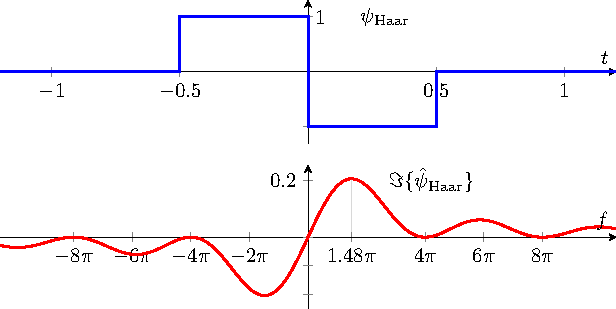
\includegraphics{papers/complex/images/haar.pdf}
	\caption{Das Haar-Wavelet (blau) und seine Hilbert-Transformierte (rot)
		\label{complex:haar}}
\end{figure}
